\documentclass{article}

\usepackage{graphicx}
\usepackage{tikz}
\usepackage{tikzsymbols}
\usetikzlibrary{calc,patterns,shapes.geometric}
\pagestyle{empty}
\usepackage[margin=0pt]{geometry}
\geometry{papersize={14in,12in}}

\def\centerarc[#1](#2)(#3:#4:#5){\draw[#1] ($(#2)+({#5*cos(#3)},{#5*sin(#3)})$) arc (#3:#4:#5);}

\begin{document}
	\begin{figure}
		\centering
		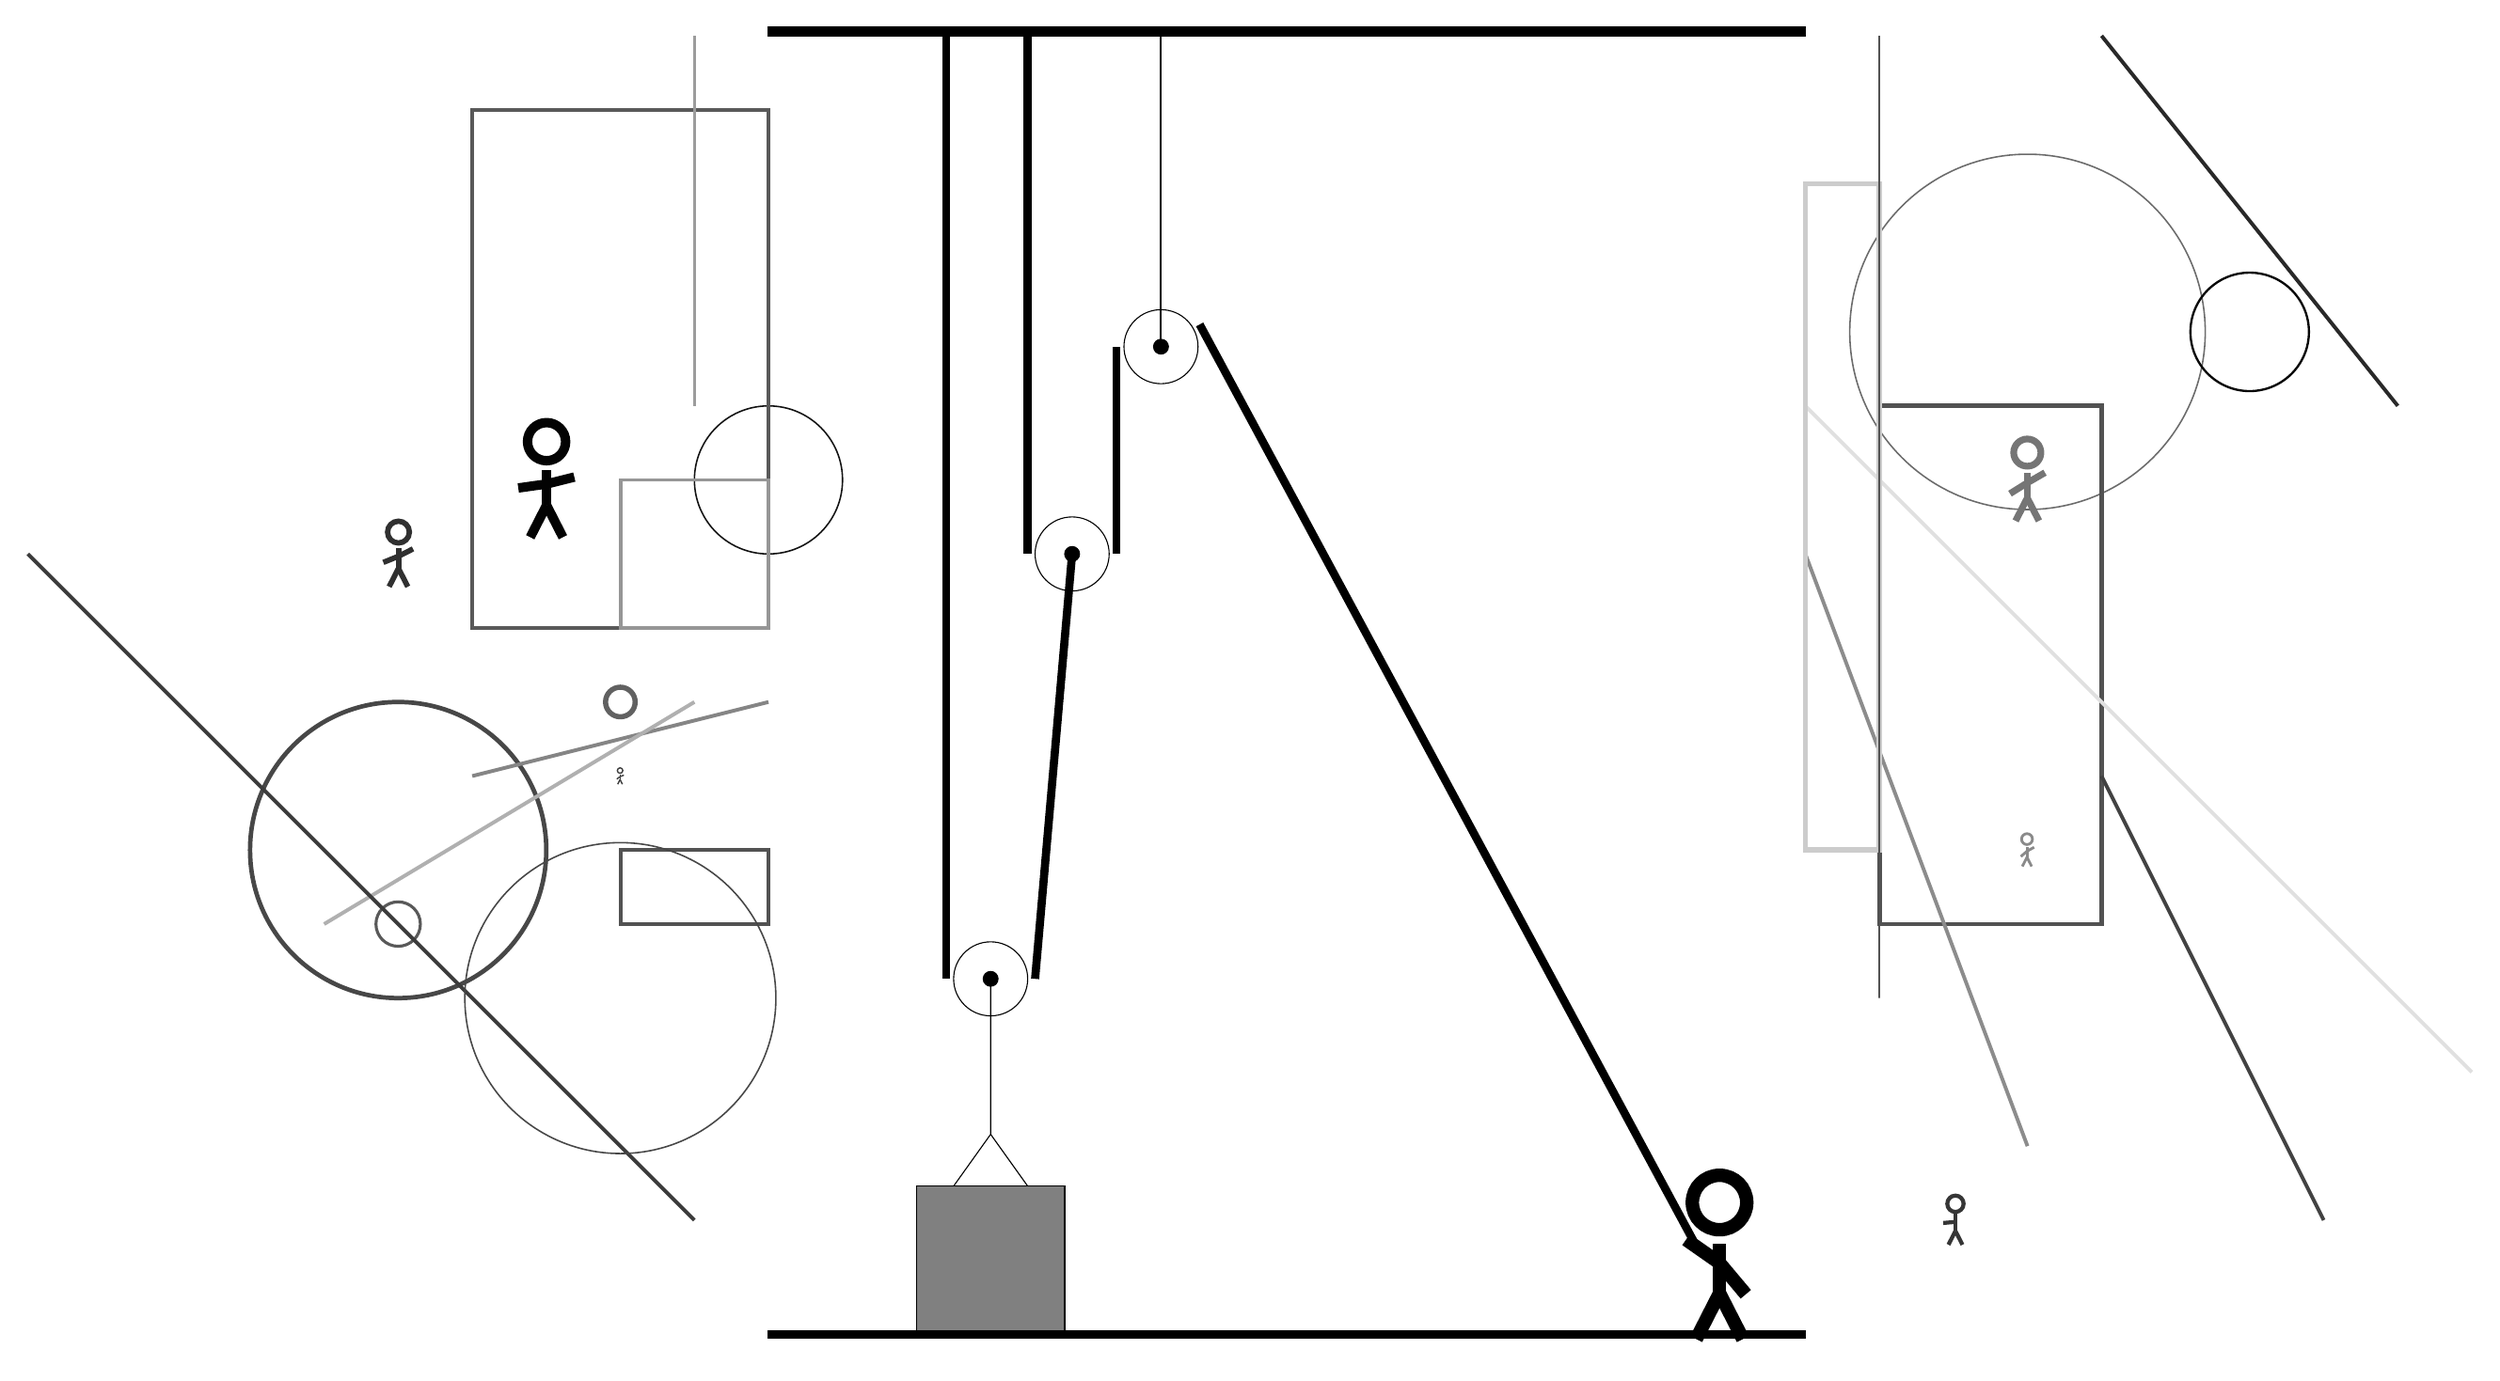
\begin{tikzpicture}
			%%%%% START %%%%%
			
			\draw[fill=black] (-2, 14) rectangle (12, 14.125);
			
			\draw (1, 1.26) circle (0.5);
			\draw[fill=black] (1, 1.26) circle (0.1);
			
			\draw (2.1, 7.0) circle (0.5);
			\draw[fill=black] (2.1, 7.0) circle (0.1);
			
			\draw (3.3, 9.8) circle (0.5);
			\draw[fill=black] (3.3, 9.8) circle (0.1);
			\draw[thick] (3.3, 9.8) -- (3.3, 14);
			
			\draw (1, 1.26) -- (1, -0.84) -- (0.5, -1.54) -- (1.5, -1.54) -- (1, -0.84);
			\draw[fill=black!50] (0, -1.54) rectangle (2, -3.54);
			
			\draw[line width=1.1mm] (0.4, 14) -- (0.4, 1.26);
			\centerarc[line width=1.1mm](1, 1.26)(180:360:0.6);
			\draw[line width=1.1mm](1.6, 1.26) -- (2.1, 7.0);
			\draw[line width=1.1mm] (1.5, 14) -- (1.5, 7.0);
			\centerarc[line width=1.1mm](2.1, 7.0)(180:360:0.6);
			\draw[line width=1.1mm](2.7, 7.0) -- (2.7, 9.8);
			\centerarc[line width=1.1mm](3.3, 9.8)(30:180:0.6);
			\draw[line width=1.1mm] (3.822, 10.1) -- (10.5, -2.3);
			
			\node at (10.8, -2.5) {\Strichmaxerl[10][-35][-50]};
			
			\draw [line width=0.7mm, color=black!62](-4, 5) circle (0.2);
			
			\draw [line width=0.2mm, color=black!58](15, 10) circle (2.4);
			\draw [line width=0.6mm, color=black!72](-7, 3) circle (2.0);
			\draw[line width=0.5mm, color=black!68] (-4, 3) rectangle (-2, 2);
			\draw[line width=0.5mm, color=black!48](-6, 4) -- (-2, 5);
			\node[line width=0.3mm, color=black!81] at (-7, 7) {\Strichmaxerl[4][22][27]};
			\node[line width=0.6mm, color=black!54] at (15, 8) {\Strichmaxerl[5][32][30]};
			
			\draw[line width=0.6mm, color=black!68] (13, 9) rectangle (16, 2);
			\node[line width=0.6mm, color=black!75] at (-4, 4) {\Strichmaxerl[1][37][21]};
			\draw[line width=0.5mm, color=black!45](15, -1) -- (12, 7);
			\node[line width=0.4mm, color=black!46] at (15, 3) {\Strichmaxerl[2][41][29]};
			\draw [line width=0.2mm, color=black!93](-2, 8) circle (1.0);
			\draw[line width=0.5mm, color=black!65] (-2, 13) rectangle (-6, 6);
			\draw[line width=0.5mm, color=black!12](12, 9) -- (21, 0);
			\draw[line width=0.7mm, color=black!20] (13, 12) rectangle (12, 3);
			\draw[line width=0.3mm, color=black!68] (13, 1) rectangle (13, 14);
			
			\draw[line width=0.5mm, color=black!84](16, 14) -- (20, 9);
			\draw [line width=0.3mm, color=black!97](18, 10) circle (0.8);
			\draw[line width=0.5mm, color=black!41] (-4, 8) rectangle (-2, 6);
			\draw[line width=0.5mm, color=black!31](-3, 5) -- (-8, 2);
			\node[line width=0.7mm, color=black!99] at (-5, 8) {\Strichmaxerl[7][8][14]};
			\draw [line width=0.4mm, color=black!65](-7, 2) circle (0.3);
			\draw[line width=0.5mm, color=black!74](16, 4) -- (19, -2);
			\draw[line width=0.4mm, color=black!39] (-3, 9) rectangle (-3, 14);
			\draw[line width=0.5mm, color=black!77](-3, -2) -- (-12, 7);
			
			\draw [line width=0.2mm, color=black!72](-4, 1) circle (2.1);
			
			\node[line width=0.6mm, color=black!79] at (14, -2) {\Strichmaxerl[3][5][90]};
			
			\draw[fill=black] (-2, -3.5) rectangle (12, -3.6);
			
			%%%%% END %%%%%
		\end{tikzpicture}
	\end{figure}	
\end{document}